\subsection{Determinant ($\det(A)$ or $\dabs{A}$)}


\begin{table}[H]
    \hfill
    \begin{minipage}{0.45\linewidth}
        \begin{figure}[H]
            \centering
            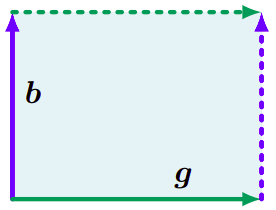
\includegraphics[
                width=\linewidth,
                height=3cm,
                keepaspectratio,
            ]{images/maths-for-ml/determinant-2d.png}
            \caption*{
                The area of the parallelogram (shaded region) spanned by the vectors $\bm{b}$ and $\bm{g}$ is $\dabs{\det([\bm{b}, \bm{g}])}$.
                \cite{mfml/book/mml/Deisenroth-Faisal-Ong}
            }
        \end{figure}
    \end{minipage}
    \hfill
    \begin{minipage}{0.45\linewidth}
        \begin{figure}[H]
            \centering
            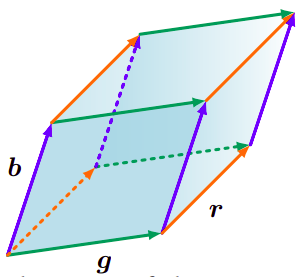
\includegraphics[
                width=\linewidth,
                height=3cm,
                keepaspectratio,
            ]{images/maths-for-ml/determinant-3d.png}
            \caption*{
                The volume of the parallelepiped (shaded volume) spanned by vectors $\bm{r}$, $\bm{b}$, $\bm{g}$ is $\dabs{\det([\bm{r}, \bm{b}, \bm{g}])}$.
                \cite{mfml/book/mml/Deisenroth-Faisal-Ong}
            }
        \end{figure}
    \end{minipage}
    \hfill
\end{table}


.\hfill
$
    \det(\bm{A}) 
    = \dabs{\bm{A}}
    = \begin{vmatrix}
        a_{11} & a_{12} & \cdots & a_{1n} \\
        a_{21} & a_{22} & \cdots & a_{2n} \\
        \vdots & \vdots & \ddots & \vdots \\
        a_{n1} & a_{n2} & \cdots & a_{nn} \\
    \end{vmatrix}
$
\hfill \cite{mfml/book/mml/Deisenroth-Faisal-Ong}

\begin{enumerate}
    \item A determinant is a mathematical object in the analysis and solution of systems of linear equations.
    \hfill \cite{mfml/book/mml/Deisenroth-Faisal-Ong}

    \item Determinants are \textbf{only} defined for square matrices $\bm{A} \in \mathbb{R}^{n\times n}$ ,i.e., matrices with the same number of rows and columns.
    \hfill \cite{mfml/book/mml/Deisenroth-Faisal-Ong}

    \item The determinant of a square matrix $\bm{A} \in \mathbb{R}^{n\times n}$ is a function that maps $\bm{A}$ onto a real number.
    \hfill \cite{mfml/book/mml/Deisenroth-Faisal-Ong}

    \item For $n=1$, $\det(\bm{A}) = \det(a_{11}) = a_{11}$
    \hfill \cite{mfml/book/mml/Deisenroth-Faisal-Ong}

    \item For $n=2$, 
    $
        \det(\bm{A}) 
        = \begin{vmatrix}
            a_{11} & a_{12} \\
            a_{21} & a_{22}
        \end{vmatrix} 
        = a_{11} a_{22} - a_{12} a_{21}
    $
    \hfill \cite{mfml/book/mml/Deisenroth-Faisal-Ong}

    \item (\textbf{Sarrus’ rule}) For $n=3$, 
    \hfill \cite{mfml/book/mml/Deisenroth-Faisal-Ong}
    \\[0.3cm]
    $
        \det(\bm{A}) 
        = \begin{vmatrix}
            a_{11} & a_{12} & a_{13} \\
            a_{21} & a_{22} & a_{23} \\
            a_{31} & a_{32} & a_{33} \\
        \end{vmatrix} 
        = a_{11} a_{22} a_{33}  + a_{21} a_{32} a_{13}  + a_{31} a_{12} a_{23}  - a_{31} a_{22} a_{13}  - a_{11} a_{32} a_{23}  - a_{21} a_{12} a_{33} 
    $
    \hfill \cite{mfml/book/mml/Deisenroth-Faisal-Ong}

    \item For a triangular matrix $\bm{T} \in \mathbb{R}^{n\times n}$ , the determinant is the product of the diagonal elements, i.e., $\det(\bm{T}) = \dsum ^n _{i=1} \bm{T}_{ii}$
    \hfill \cite{mfml/book/mml/Deisenroth-Faisal-Ong}

    \item the determinant $\det(\bm{A})$ is the signed volume of an n-dimensional parallelepiped formed by columns of the matrix $\bm{A}$.
    \hfill \cite{mfml/book/mml/Deisenroth-Faisal-Ong}

    \item The sign of the determinant indicates the orientation of the spanning vectors.
    \hfill \cite{mfml/book/mml/Deisenroth-Faisal-Ong}

    \item \textbf{Theorem} (Laplace Expansion): Consider a matrix $\bm{A} \in \mathbb{R}^{n\times n}$. Then, for all $j = 1, \cdots , n$:
    \hfill \cite{mfml/book/mml/Deisenroth-Faisal-Ong}
    \begin{enumerate}
        \item Expansion along column $j$: 
        $
            \det(\bm{A}) = \dsum^n _{k=1} (-1)^{k+j}\  a_{kj}\ \det(\bm{A}_{k,j} )
        $
        \hfill \cite{mfml/book/mml/Deisenroth-Faisal-Ong}

        \item Expansion along row $j$:
        $
            \det(\bm{A}) = \dsum^n _{k=1} (-1)^{k+j}\  a_{jk}\ \det(\bm{A}_{j,k} )
        $
        \hfill \cite{mfml/book/mml/Deisenroth-Faisal-Ong}

        \item $\bm{A}_{k,j} \in \mathbb{R}^{(n-1)\times(n-1)}$ is the sub-matrix of $\bm{A}$ that we obtain when deleting row $k$ and column $j$.
        \hfill \cite{mfml/book/mml/Deisenroth-Faisal-Ong}

        \item $\det(\bm{A}_{k,j} )$ is called a \textbf{minor} and $(-1)^{k+j}\ \det(\bm{A}_{k,j} )$ a \textbf{cofactor}.
        \hfill \cite{mfml/book/mml/Deisenroth-Faisal-Ong}
    \end{enumerate}

\end{enumerate}



\begin{lstlisting}[
    language=Python,
    caption=Determinant of matrix - numPy
]
import numpy as np

# Define a square matrix
A = np.array([
    [1, 2],
    [3, 4]
])

# Compute the determinant
det_A = np.linalg.det(A)

print("Matrix A:\n", A)
print("Determinant of A:", det_A)
\end{lstlisting}




\subsubsection{Properties of Determinant}

For $\bm{A} \in \mathbb{R}^{n\times n}$ the determinant exhibits the following properties:
\hfill \cite{mfml/book/mml/Deisenroth-Faisal-Ong}

\begin{enumerate}
    \item The determinant of a matrix product is the product of the corresponding determinants, $\det(\bm{AB}) = \det(\bm{A})\det(\bm{B})$.
    \hfill \cite{mfml/book/mml/Deisenroth-Faisal-Ong}

    \item Determinants are invariant to transposition, i.e., $\det(\bm{A}) = \det(\bm{A}^\top)$.
    \hfill \cite{mfml/book/mml/Deisenroth-Faisal-Ong}

    \item If $\bm{A}$ is regular (invertible), then $\det(\bm{A} ^{-1} ) = \dfrac{1} {\det(\bm{A})}$.
    \hfill \cite{mfml/book/mml/Deisenroth-Faisal-Ong}

    \item Similar matrices possess the same determinant. 
    Therefore, for a linear mapping $\Phi : V \to V$ all transformation matrices $\bm{A}_\Phi$ of $\Phi$ have the same determinant. 
    Thus, the determinant is invariant to the choice of basis of a linear mapping.
    \hfill \cite{mfml/book/mml/Deisenroth-Faisal-Ong}

    \item Adding a multiple of a column/row to another one does not change $\det(\bm{A})$.
    \hfill \cite{mfml/book/mml/Deisenroth-Faisal-Ong}

    \item Multiplication of a column/row with $\lambda \in \mathbb{R}$ scales $\det(\bm{A})$ by $\lambda$. 
    In particular, $\det(\lambda \bm{A}) = \lambda^ n \ \det(\bm{A})$.
    \hfill \cite{mfml/book/mml/Deisenroth-Faisal-Ong}

    \item Swapping two rows/columns changes the sign of $\det(\bm{A})$.
    \hfill \cite{mfml/book/mml/Deisenroth-Faisal-Ong}

    \item[] \textbf{Note}: Because of the last three properties, we can use Gaussian elimination to compute $\det(\bm{A})$ by bringing $\bm{A}$ into row-echelon form. 
    We can stop Gaussian elimination when we have $\bm{A}$ in a triangular form where the elements below the diagonal are all $0$. 
    (the determinant of a triangular matrix is the product of the diagonal elements)
\end{enumerate}









